\graphicspath{{pro-ndi/}}

\chapter{Learning Representative Climate-Relevant Numbers}
\label{chap:prondi}

The Numerically-Driven Inferencing (NDI) paradigm is introduced in Section~\ref{sec:ndi}.
In Chapters~\ref{chap:two} and \ref{chap:evilndi}, we have seen further
demonstrations of the kinds of marked attitudinal and conceptual shifts one can
obtain with quite minimalist interventions. In particular, we've seen the
striking effects of the EPIC procedure (both introduced by
\nptextcite{ranney_numerically_2001_fixed}), as well as more minimal
interventions involving only the “E” (Estimate) and “I” (Inform) portions of the
EPIC intervention. (\nptextcite{rinne_estimation_2006}, also explore the primary
importance of committing to an estimation prior to receiving the correct
information.)

As with Chapter~\ref{chap:evilndi}, we again present a collection of NDI
interventions in a somewhat different order than they were actually performed
in. This way, we are able illustrate a potential problem---specifically, even
these more representative numbers yield erosion
of confidence in one's own knowledge, just as with the “evil” numbers in
Chapter~\ref{chap:evilndi}. We'll proceed to demonstrate that this problem is solved in
Chapter~\ref{chap:mechanism}.  In the studies below, we presented participants
in the different conditions with numerical information that is relevant to
global climate change acceptance.  Unlike in Chapter~\ref{chap:evilndi}, we used
numbers that were likely to \emph{boost} acceptance. As before, survey methods employed
in the following studies are described in detail in Chapter~\ref{chap:survey}.

\section{Study 1: Online Experiment with UC Undergrads}
\label{sec:pro-uc}

Given the efficacy of “evil” numbers and previous successes of the NDI paradigm,
this study assessed the efficacy of numbers that support the claim(s) of global
climate change. Again partly tongue-in-cheek, we call these “saintly” numbers.
Given prior NDI studies of similarly “shocking” magnitudes
\parencite[e.g.,][]{garcia_de_osuna_qualitative_2004}, our hypothesis was that
the accurate feedback would increase participants’ climate change acceptance,
but diminish self-confidence in their knowledge of the issue.


\subsection{Methods}

\subsubsection{Participants}

UC Berkeley undergrads ($N=60$) were recruited via the Research Participation
Pool (RPP). Prior to engaging in experiments in the RPP program, many
participants complete a pretest screening survey containing demographics and
other items contributed by numerous experimenters. This RPP pretest was
completed by 30 of our participants. 

\subsubsection{Materials and procedure}

This study used an on-line version of materials otherwise similar to those used
in our “evil” NDI study (reported in Section~\ref{sec:evilndi-methods}), and
used a pretest survey included in the RPP screening survey. In particular, the
core intervention in which all participants were engaged was analagous to the
eight-item blast shown in Figure~\ref{fig:evil-flow}. Some participants,
however, also completed a pretest (at an earlier time during RPP prescreening).
Thus, 30 participants completed a full “sandwich” while the other 30 were in a
no-pretest condition. 

For those sandwich participants that completed the pretest, it was completed, on
average, 18 days prior to the intervention. In the main intervention, we queried
individuals about eight quantities (listed in Table~\ref{table:pro-numbers1} in
the Appendix). The eight items were accompanied by questions directed at
participants’ surprise and their reactions to each number.  Fictitious monetary
policies were left out of this version, as simple attitude shifts were readily
observed in the simplified 8-item “evil” intervention, and these shifts are more
directly comparable across experiments.  An added feature of the online
intervention is that we could remind individuals of the estimates they gave on
the same page on which they incorporated numerical feedback, ensuring that they
contrasted the two. As with online surveys in Chapter~\ref{chap:mechanism}, a
posttest regarding participant attitudes and beliefs was administered both
immediately after our intervention and after a retention interval.


% \subsubsection{Analysis}
% 
% Analyses here were largely analagous to those described in
% Section~\ref{sec:mech-online-methods}.

\subsection{Results}

\subsubsection{\emph{Self-rated} knowledge and surprise}

These items were, as anticipated and as with the “evil” items, able to
significantly erode self-rated knowledge (5.3 to 4.0 on a 1--9 scale for our full sandwich
condition, $t(29)=-3.6$, $p<0.01$).  This erosion was comparable to that found
with the “evil” numbers.  The numerical items ranked relatively high on
participant surprise compared to the (significantly effective) 400-word
mechanism intervention from Chapter~\ref{chap:mechanism}.  The mean surprise
rating across items was 4.8 (on a 1--9 scale; all ratings above “1” indicate
some level of surprise).  While this is a bit lower than surprise ratings for
“evil” numbers in Chapter~\ref{chap:evilndi}, it markedly exceeds the mean 2.9
surprise rating for the 400 words obtained using an analogous online
intervention with UC Berkeley undergrads (reported in
Section~\ref{sec:uc-online-results}). It is also very much in line with the 4.7
mean surprise rating noted in Study 2, which \emph{did} obtain attitude shifts
using very similar estimation items (reported under “Participants” in
Section~\ref{sec:CCO-ndi-methods}). Thus, the immediate affective impact of
these numbers was reported as \emph{higher} than an intervention that (as we'll
see in Chapter~\ref{chap:mechanism}) effectively supported significant shifts in
attitudes for both students and the general public.

One of the most surprising numbers (with a mean surprise rating of 5.2) was the percentage of active
researchers who support the tenets of anthropogenic climate change, reflective
of the strong relationship between perceived scientific consensus and the acceptance
of climate change reported in \textcite{lewandowsky_pivotal_2013}. The two
numbers most comparable to the statistics in the 400 words (and in the video
adaptation available at \url{http://HowGlobalWarmingWorks.org}) were similarly
surprising, with the rises in atmospheric methane and atmospheric CO2 ranking at
5.9 and 5.1, respectively---both higher than the mean surprise ratings from the
400 words in Chapter~\ref{chap:mechanism}.


\subsubsection{Global warming (GW) attitutudes}

In spite of the powerful impacts described above, attitudes, acceptance, and
beliefs regarding climate change remained stable after this intervention with
“saintly” numbers (6.71 pre versus 6.67 posttest).  This lack of effect is
counter to prior NDI studies (as well as the results reported in
Chapter~\ref{chap:mechanism}), in which individuals’ preferences and beliefs
were often markedly shifted by even a single number. 

\subsection{Discussion}


An experimental silver lining here is the demonstration that participants will
not report greater climate change acceptance merely by dint of experimenter
demand.  In both this \emph{and} previous NDI and RTMD studies, participants
were explicitly told that all feedback statistics and other information were
fully accurate, that the study involved \emph{no} deceptions.  One possible
explanation is due to a methodological change: prior studies 
also provided the particular scientific/literature source both
for each statistic that was sought and each provided as feedback.
Sources were not uniformly provided in this study. This is one
difference that may partially account for our lack-of-effect.

So, it is possible that participants were less compelled by the authority of
this study’s statistics, compared to those in Chapter~\ref{chap:evilndi}.
Another possibility is that, as in Chapter~\ref{chap:evilndi}, participants were
left feeling less knowledgeable---perhaps weakening any boost these surprising numbers
could have on climate change acceptance.  

A final possiblity is that the effect of this numerical intervention would be
strengthened by an appropriate context for integrating this information. That
is, perhaps we could not simply present our numerical information as it was in
isolation with the expectation of an effect. Indeed, as we report in
\parencite{clark_knowledge_inpress}, similar numbers had little immediate effect on
high-school students as a part of a global warming mechanism curriculum.
However, students exposed to numbers like those in this study retained the
effects of the curriculum to a greater extent than students in a control
condition.

A possibility that will disconfirmed in the introduction to the following
section is that this lack of result was due to the delay between attitudes
assessed during during RPP prescreening and our core intervention. As we'll
shortly see, this lack-of-result was replicated within a single session
intervention.

\section{Study 2: Online intervention with Amazon Mechanical Turk}
\label{sec:pro-mturk}

After the difficulty obtaining shifts in GW attitudes and beliefs above, I was
able to replicate this difficulty by presenting the same materials to a more
general population on Amazon Mechanical Turk. I won't go through the
exercise of reporting another null result here, apart from mentioning that
unlike the above, this intervention contained a full “sandwich” in a single
survey/session. Thus, it seems unlikely that our difficulty in observing a
result with these particular materials depends on the timing of the pretest.

I then engaged in a thorough examination of the wording of the items (also
discovering that the informational feedback for one item was off by an order of
magnitude due to an error converting from the metric system).  This process was
relatively informal, and consisted of showing the items to naïve individuals and
asking them if they had any difficulty understanding them.  Descriptions were
iterated until they appeared to make sense to non-experts.

\subsection{Methods}
\label{sec:CCO-ndi-methods}

\subsubsection{Participants}

“Workers” on the Amazon Mechanical Turk platform ($N=40$) were recruited to
complete a two-part survey. Language used in recruitment made no mention of
climate change, and was titled “Politics, Numbers, and Your Attitudes.” After
removal of problematic participants above, we were left with 38 participants in
the intervention. Eighteen of the total retained participants were female. One
participant reported being born outside the United States, but residing here for
20 years. Mean conservativism was 4.0 on a 1--9 scale
($sd=2.1$), which is comparable with our college students in other studies in
this dissertation. However, participants in this study were more likely to
declare being a Democrat or Republican.  While the sample is still clearly
biased towards the Democratic/liberal end of the political spectrum, the ratio
between Republicans and Democrats is less extreme than our undergraduate
samples. This is in line with the results reported by
\textcite{richey_how_2012}, in which approximately 73\% of polled workers on
Mechanical Turk reported voting for Obama (versus approximately 51\% in the
election results).  The complete distribution of declared political party
affiliation is reported in Table~\ref{table:CCO-ndi-party}.

% latex table generated in R 2.15.1 by xtable 1.7-1 package
% Fri Jun 21 16:05:32 2013
\begin{table}[ht]
    \caption{Number (and percentage) of individuals declaring a given party
        affiliation.}
    \label{table:CCO-ndi-party}
\centering
\begin{tabular}{rcc}
  \toprule
      & party (percentage) \\ 
  \midrule
  democrat &  17 (44.7) \\ 
  independent &  12 (31.5) \\ 
  republican &   4 (10.5) \\ 
  libertarian &   3 (7.8) \\ 
  other &   1 (2.6) \\ 
  decline to state &   1 (2.6) \\ 
  \midrule
  total &  38 (100.0) \\ 
   \bottomrule
\end{tabular}
\end{table}

% This is a spurious result, as our own demographics didn't separate protestants
% and catholics
% A final interesting feature of our population is that all participants reporting
% their faith as Christian self-identified as Catholic. That is, we had no
% “protestant” participants.

\subsubsection{Materials and procedure}

Materials are largely identical with those in Study 1, apart from the
improvements in comprehensibility described above. An additional improvement in
terms of making the survey more clear was replacing a fill-in-the-blank question
for specifying units and “increase” or “decrease” for their estimate. In this
version of the experiment, one or two choices including the unit and direction
were provided as appropriate to each estimate. For example, “\% of researchers”
or “feet increase.” The item reproduced in Appendix~\ref{app:format-ndi} is an
exact copy of the format used for this study.  Note that participants were
further asked to indicate their experience of an item on three different
scales---one asking about “surprise,” one about “embarrassment at lack of
knowledge,” and one about the familiarity of the item.

On inspecting the materials used in Study 1, numerous individuals remarked that
the instructions were too long, and the materials difficult to understand. Thus,
for this study, I endeavored to eliminate unnecessary instructions and generally
simplify language. This was a somewhat subjective process, but feedback from
non-experts indicated that the materials used in this study were indeed easier
to understand. Note that in the process of streamlining instructions, I removed
instructions to the effect that \emph{no} deceptions were used. This is in
contrast to the previous (ineffective) study that did include such an
instruction.  In addition, in this study even more than in the above study, the
inclusion of information about authority was scant (e.g., the more accessible
phrase “journal article” replaced phrases such as “article published in PNAS”).
The correct trade-off between simplicity and completeness (e.g., inclusion of
proper references) is a worthy topic of further consideration.  The exact
wording used in this study is shown in Table~\ref{table:pro-numbers2} in the
Appendix.

A final change was the removal of an item on sea-level rise, the feedback for
which had previously been incorrectly reported as 10 times higher than the true
amount. It is a small possibility that this item undermined individual's belief
in our other numbers in Study 1 above, but based on comments, only a few
individuals appeared to doubt the number.

\subsubsection{Data quality on Amazon Mechanical Turk}
\label{sec:mturk-problems}

The use of an anonymous, on-line labor pool raises concerns about data quality.
For example, people may try to take the survey again or they may lie about their
demographics (i.e., claiming they are U.S. residents so that they may gain the
credit). Re-taking is one of the most easily guarded against concerns on Amazon
Mechanical Turk, as Amazon will attempt to enforce this if requested, as was
done in this study. However, in addition, no IP addresses were repeated in the
participant pool for this study.

Amazon will attempt to restrict individuals to the U.S. if requested, and this
was done for this experiment. An additional layer of verification of location is
straightforward using “geo IP” databases. In this case, geographical locations
were retrieved using the GeoLite data created by MaxMind (available from
\url{http://www.maxmind.com}). On our survey, participants indicated the state
they reside in. Participant IP addresses were subsequently checked against this
reported location. Here, two individuals IP’s appeared to be located in Germany
and Guatemala, and so these participants were excluded. Most other
participants had IP addresses that resolved to the state they claimed to be
from. One participant’s IP address was not listed in the MaxMind database, and
was traced to either Hughes Net or Bright Home, both U.S.-only satellite
internet providers.

\subsection{Results}

\subsubsection{Surprise and related measures}

The numerical feedback was again ranked as surprising, and in a similar range to
that observed in the above Study (which failed to shift attitudes). Here, we
have a total of 21 measures of something like surprise, three for each of our
seven estimation items.  The number of potential relationships is large here, so
we must be cautious in over-interpreting \emph{post hoc} observation. However,
some clear structure appears to exist amongst these correlations, as can be seen
in Figure~\ref{fig:CCO-prondi-surp-corr}. Specifically, we can observe a clear
block structure near the diagonal for the “embarrassment” and familiarity
ratings.\footnote{“Block structure” is a common notion used in mathematics when
    describing a square region of a grid, where the elements of that region are
    more similar to each other than to some other portion of the grid. Here, the
    grid is displayed as a bitmap in Figure~\ref{fig:CCO-prondi-surp-corr}, but
    it could just as easily be represented as a matrix of numbers. In either
    case, the term “block structure” would be appropriate} It seems that
individuals had a tendency to rate these items relatively low or high across
items (reflected by larger off-diagonal correlations), while such correlation
was not present with “surprise” (i.e., ratings of surprise tended not to predict
one another within a given participant). This can be summarized statistically with the
averages of the off-diagonal correlations in these blocks. The surprise items
had a mean correlation with each other of 0.14, while the embarrassment and
familiarity items had means of 0.41 and 0.40, respectively.

Another clear structure can be seen in the smaller diagonals visible off the
main diagonal.  Where these diagonals appear, this indicates that for a given
item, the relevant measures tended to covary. The mean of the correlations along
these minor diagonals were as follows: surprised with embarrassed was 0.57,
surprised with familiar was -0.31, and embarrassed with familiar was -0.09.
Thus, embarrassment and familiarity do a poor job of (anti-)predicting one another.
Surprise, however, is well correlated with the embarrassment rating, and still
reasonably (anti-)correlated with familiarity. 

Please note that above, we are not engaged in a process of hypothesis testing,
as these correlations are of little import for our hypothesis-driven
conclusions. Rather, these correlations should be interpreted as descriptive
measures to assist with the comprehension of the structure in this data (and
potentially inspire future hypothesis-driven research).

\begin{figure}
    \centering
    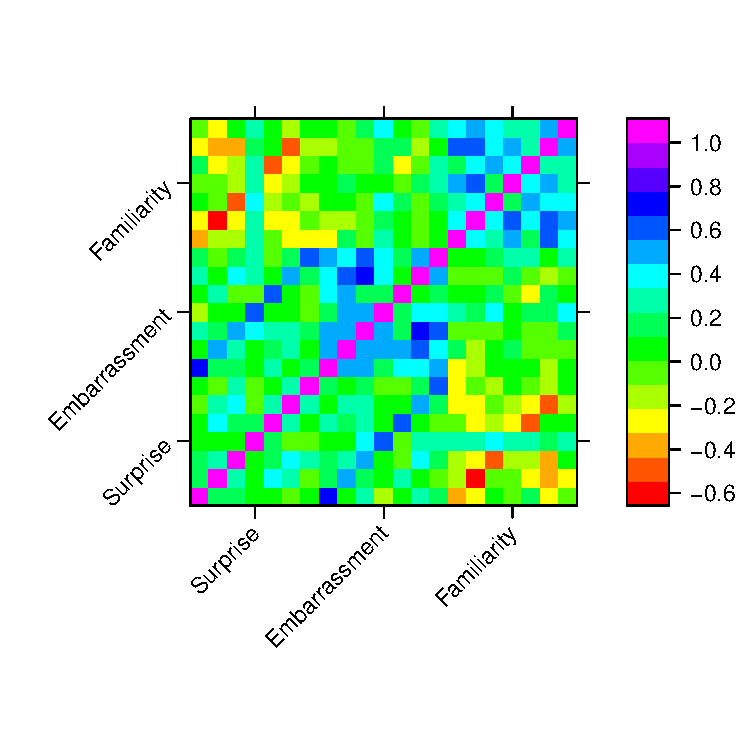
\includegraphics{CCO-prondi-surp-corr.pdf}
    \caption{An image plot of the correlations between ratings for each of the 3
        ratings across the 7 estimation items (note that the plot is symmetric,
        such that all off-diagonal correlations are included twice). Each rating
        type is presented in a seven-item block centered vertically and
        horizontally on one of the three labels (textual labels apply to all
        items within a seven-by-seven block).  Relatively clear block structure
        is apparent surrounding the main diagonal for embarrassment and
        familiarity (specifically, there are more blue/high correlation values
        in these seven-by-seven blocks).  Parallel to the main diagonal, a
        blue/high correlation diagonal of positive correlations can be seen
        within an item between embarrassment and surprise, and a red/negative
        correlation diagonal can be seen for surprise and familiarity.}
    \label{fig:CCO-prondi-surp-corr}
\end{figure}

Across items, surprise ranged from 3.2 to 6.3 ($\mu=4.7$), embarrassment from
2.6 to 4.3 ($\mu=3.4$), and familiarity from 2.9 to 4.1 ($\mu=3.6$). (All items
were rated on a 1--9 scale.) Some floor effects may have occurred for embarrassment
and familiarity (the opposite of what we'll see in Chapter~\ref{chap:mechanism}.
If we order our items by one of these ratings, the order remains the same if we
use surprise or embarrassment (but the order changes for familiarity). 

Overall, it appears that our surprise question is the least likely to be
uniformly high or low across items for a given subject, thus the variation in
responses to this item is more likely to be reflective of an individual's
response to the item itself. For these numbers, surprise also suffers from less of a
floor effect. That said, no combination of mean or maximum surprise (and
related) scores were significantly predictive of shifts in GW acceptance and
concern.

\subsubsection{GW acceptance supported by clear numerical information}

This version of the intervention did significantly boost mean GW acceptance and
concern by about 1/3 of a point from a pretest mean of 6.4 to a posttest mean of
6.8, as depicted in Figure~\ref{fig:prondi-gw}. The shift was significant
($t(37) = 2.74$, $p < 0.01$). Thus, it appears that while we (and others)
experience some failures of numeracy to achieve shifts in the direction of
scientific consensus, it appears that a carefully crafted intervention can have
useful effects.

\begin{figure}
    \centering
    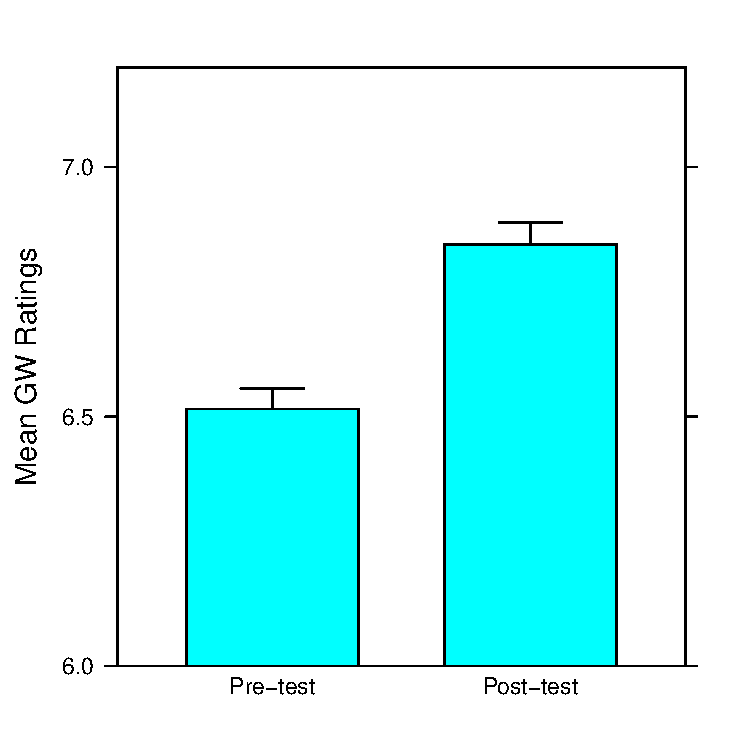
\includegraphics{CCO-prondi-gw.pdf}
    \caption{Shifts in GW ratings in Mechanical Turk intervention with
        climate-change-supporting numbers. The pretest mean is 6.4 and the
        posttest mean is 6.8.}
    \label{fig:prondi-gw}
\end{figure}

\subsubsection{Self-confidence in GW knowledge is still eroded}

While we see shifts above towards the scientific consensus on global warming,
participants still report feeling about a point less knowledgeable (dropping
from a pretest mean of 5.2 to a posttest mean of 4.2) as depicted in
Figure~\ref{fig:prondi-knw}. This drop is significant ($t(37)=-3.38$, $p<0.001$).

\begin{figure}
    \centering
    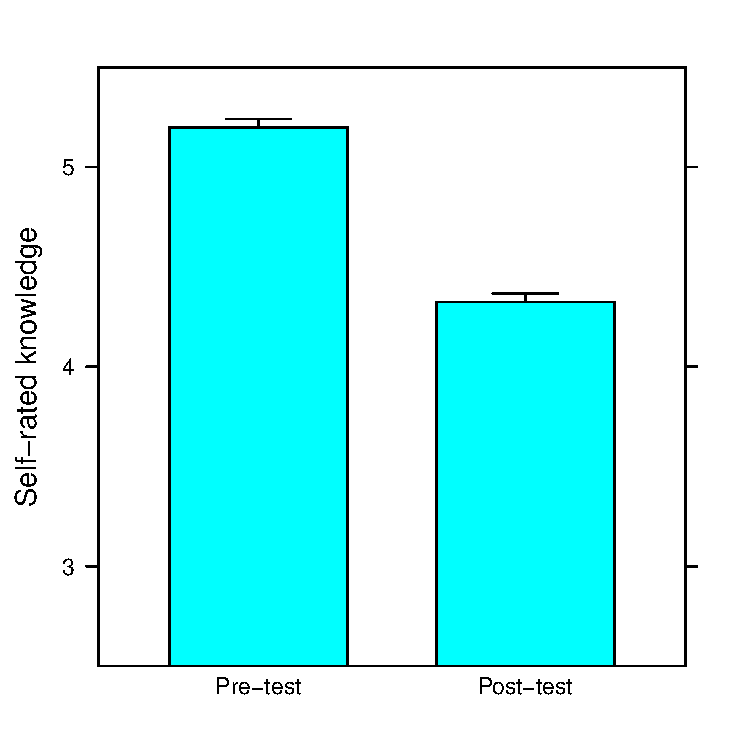
\includegraphics{CCO-prondi-knw.pdf}
    \caption{Erosion of confidence in self-ratings of GW knowledge in Mechanical
        Turk intervention with climate-change-supporting numbers. Means are 5.2
    on the pretest and 4.2 on the posttest.}
    \label{fig:prondi-knw}
\end{figure}

% \subsubsection{No observed effect of political variables}
% 
% TODO?
% With this sample, we are able to examine the effects of
% conservativism or political party. Figure XXX shows attitudes broken out by
% Republican, Democrat (and Other).

\subsection{Discussion}

As compared with Study 1, the primary changes were a different target population
and a modification to improve the comprehensibility of our materials. While
there were differences in declared party affiliation, conservativism was quite
similar between this group and other student populations. It should be noted,
however, that our undergraduates' mean GW ratings on the pretest were a bit high
compared to our other interventions with undergrads (and comparable to some
posttest scores!). Thus, there may have been a ceiling effect. Regarding the
materials used in this study, they seemed more comprehensible to non-experts (at
least informally). As such, this intervention may have been more persuasive in
shifting participants' acceptance of climate change and related attitudes. We
should be careful, however, in making comparisons across populations with
different interventions.  If one were truly interested in the effect of
materials, one should provide the materials as used in Studies~1 and 2 to the
same target population. If one is uninterested in such questions about
materials, I'd recommend the materials from Study~2, perhaps with the addition
of a statement about “no deceptions being used”. The basic “saintly” information
communicated in both sets of materials was quite similar.

The similarity in the effects reported in Chapter~\ref{chap:mechanism} provide
some evidence that similar interventions perform similarly across UC Berkeley
undergrads and workers on Mechanical Turk.  Thus, it seems reasonable to
recommend that careful attention be given to materials like those used in this
chapter. Items should be tested for comprehensibility with naïve individuals
prior to attempting to use them in a belief change or behavioral change
intervention. Again, the optimal balance of simplicity and completeness is a
topic for future study.

Note also that, for reasons of time and simplicity, we did not include policy
shifts in this study. However, we can still compare the size of belief and
attitude shifts with the 2-item study described in Chapter~\ref{chap:evilndi}
and infer that we are seeing attitudinal shifts of a similar magnitude.

\section{Summary and Conclusions}

Despite the lack of any observed (even numerical) shift in GW beliefs and
attitudes in Study 1 above, it affords us a number of insights.  Critically, we
cannot simply throw a set of statistics at Americans and expect that to impact
their beliefs and attitudes. While we cannot claim to know for sure what “went
wrong” with Study 1, there are a few notable differences.  In both studies, not
all items had sources, but sources were further simplified (and sometimes
omitted) in Study 2. Many were likely difficult to understand in Study 1
(wordings in Appendix~\ref{app:numbers} are reflective of the final wordings
used in Study 2). Unlike Study 2, Study 1 \emph{did} include the assertion that
the study involved no deceptions. Thus, an obvious possible explanation is that
a certain degree of comprehensibility may be necessary to effect shifts in GW
attitudes and beliefs. A final possibility is that this lack-of-effect occurred
because of a ceiling effect.  But in any case a real silver lining here is
support for the conclusion that shifts, when we do observe them, are \emph{not}
driven merely by experimenter demand.

Combined with Chapter~\ref{chap:evilndi}, we have now witnessed numeracy-based
interventions that push individuals towards and away from the scientific
consensus on anthropogenic climate change. In addition, we have seen that even
when students claim surprise regarding a set of numbers, they may not be
influenced by these numbers---unless perhaps they are presented with the
necessary clarity.

It should be noted also that, as in Chapter~\ref{chap:evilndi}, participants were
left feeling less knowledgeable than they reported prior to the intervention. It
remains for future research to determine what impact this might have on
behavior, but it seems likely that a lack of confidence would likely
inhibit public statements or commitments regarding climate change.

Our research group has also integrated such numbers with  more comprehensive
interventions. For example, \textcite{clark_knowledge_inpress} reports on the
utility of such numbers in improving retention of a climate change curriculum
described in \textcite{felipe_numerical_2012}. In the following chapter, we'll
see another relatively simple, but more comprehensive intervention that includes two
of our more surprising numbers. This intervention leaves participants both more informed
\emph{and} more confident in their own knowledge.

\section*{Acknowledgements}

The work reported in this chapter has been previously published, in part, in
\textcite{clark_knowledge_inpress}.  All such material is re-used here with the
permission of my co-authors, the publishers, and the Graduate Division at the
University of California, Berkeley.
